\newcommand{\class}[1]{\texttt{#1}}
\newcommand{\method}[1]{\texttt{#1}}
\newcommand{\attr}[1]{\textit{#1}}

Im Folgenden werden einige Designentscheidungen des Projekts beschrieben.
Dazu werden zuerst die entworfenen Klassen mit deren Attributen und Methoden beschriebenen.
Danach werden einige Verhaltensaspekte mit Sequenzdiagramm veranschaulicht.

\subsection{Struktur}
Diagramm \ref{fig:class_diagramm} zeigt alle Klassen mit deren Beziehungen, Attributen und Methoden.


\begin{figure}[htbp]
	\centering
	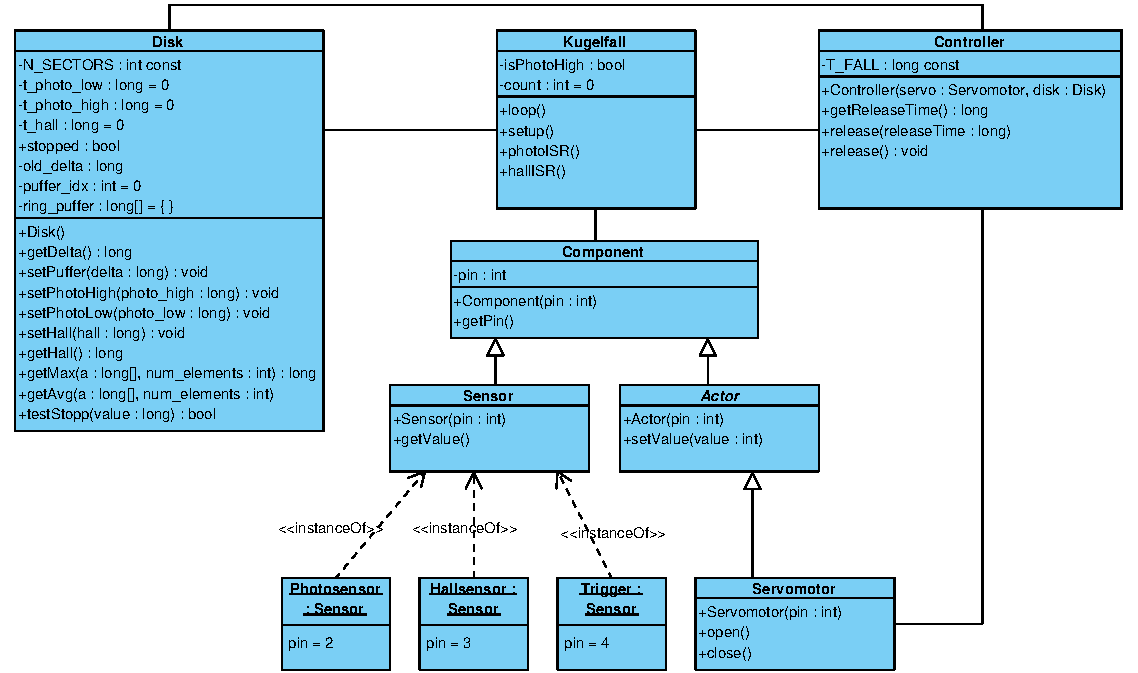
\includegraphics[width=\textwidth]{abb/class_cropped}
	\caption{Klassen mit deren Beziehungen, Methoden und Attributen}
	\label{fig:class_diagramm}
\end{figure}

\paragraph{\class{Kugelfall}}
ist die zentrale Klasse, da sie die Arduino-Methoden \method{setup()} und \method{loop()} enthält.
Sie steht in Beziehung zur allen anderen Klassen.
Innerhalb der \method{setup()}-Methode initialisiert sie die anderen Projekt-Klassen mit den entsprechenden Parametern (siehe Diagramm \ref{fig:setup_diagram}).
Ebenso werden die Interrupts zum Photosensor und Hallsensor mit den Methoden \method{photoISR()} bzw. \method{hallISR()} initialisiert (siehe Diagramm \ref{fig:photoISR} und \ref{fig:hallISR}).
Innerhalb der \method{loop()}-Methode wird auf Triggerdruck des Nutzers gewartet und ggf. der Mechanismus zur Berechnung der Fallzeit und das Loslassen aufgerufen (siehe Diagramm \ref{fig:loop_diagram}).

\paragraph{\class{Component}} entspricht einer Hardware-Komponente, auf welche mittels Arduino zugegriffen werden kann.
Es besitzt als einziges Attribut den \attr{pin} der Arduino-Kompoente, welcher im Konstruktor initialisiert wird und mittels der Funktion \method{getPin()} abgerufen werden kann.

\paragraph{\class{Sensor}} entspricht einem Hardware-Sensor und ist eine Spezialisierung der Klasse \class{Component}. 
Es initialisiert die Instanz mit dem Pin-Modus \texttt{INPUT\_PULLUP} und dem übergebenen Pin.
Die Methode \method{getValue()} liest zur Aufrufzeit den entsprechenden Wert aus.
Dabei gibt es bei diesem Projekt insgesamt die drei Sensor-Exemplare \textit{Photosensor}, \textit{Hallsensor} und \textit{Trigger}, die jeweils mit den entsprechenden Pins initialisiert wurden. 

\paragraph{\class{Actor}} entspricht einem Hardware-Aktor und ist eine Spezialisierung der Klasse \class{Component}.
Es initialisiert die Instanz mit dem Pin-Modus \texttt{OUTPUT} und dem übergebenen Pin.
Die Methode \method{setValue()} schreibt den übergebenen Wert zum Aktor.

\paragraph{\class{Servomotor}} entspricht einem Hardware-Servomotor und ist eine Spezialisierung der Klasse \class{Actor}.
Es initialisiert im Konstruktur den Servomotor mit dem entsprechenden Pin.
Die Methoden \method{open()} und \method{close()} dienen zum Öffnen und Schließen des Servomotors und damit der Fallvorrichtung.

\paragraph{\class{Disk}} entspricht der Scheibe des Kugellfallaufbaus.
Neben festen Spezifikationen wie die Anzahl der Sektoren und der Lochlänge hat es auch die Attribute zum Festhalten der letzten Zeiten für des Photo- und Hallsensors. 
Zur Speicherung der Werte des Delta-Werte des Photosensor nutzt es einen Ringpuffer, sodass die 20 zuletzt ermittelten Werte gespeichert werden.
So kann auf Fehler durch Messungenauigkeiten reagiert werden.
Zudem enthält es Funktionen der Geschwindigkeit der Schreibe auf Basis der Sensorenzeiten.

\paragraph{\class{Controller}} dient zur Berechnung der Fallzeit und dem Loslassen der Kugeln.
Zur Berechnung der Fallzeit benutzt sie die feste Fallzeit der Kugel \attr{T\_FALL} und die Geschwindigkeitsberechnungen der Klasse \class{Disk} (näheres siehe \ref{ssec:nutzung}).
Für das Fallenlassen nutzt es die Klasse \class{Servomotor}.

\subsection{Verhalten}
Im Folgenden werden einige Verhaltensaspekte beschrieben.

Diagramm \ref{fig:setup_diagram} zeigt die Initialisierung der Anwendung mittels der Methode \method{setup} der Klasse \class{Kugelfall}.
\begin{figure}[htbp]
	\centering
	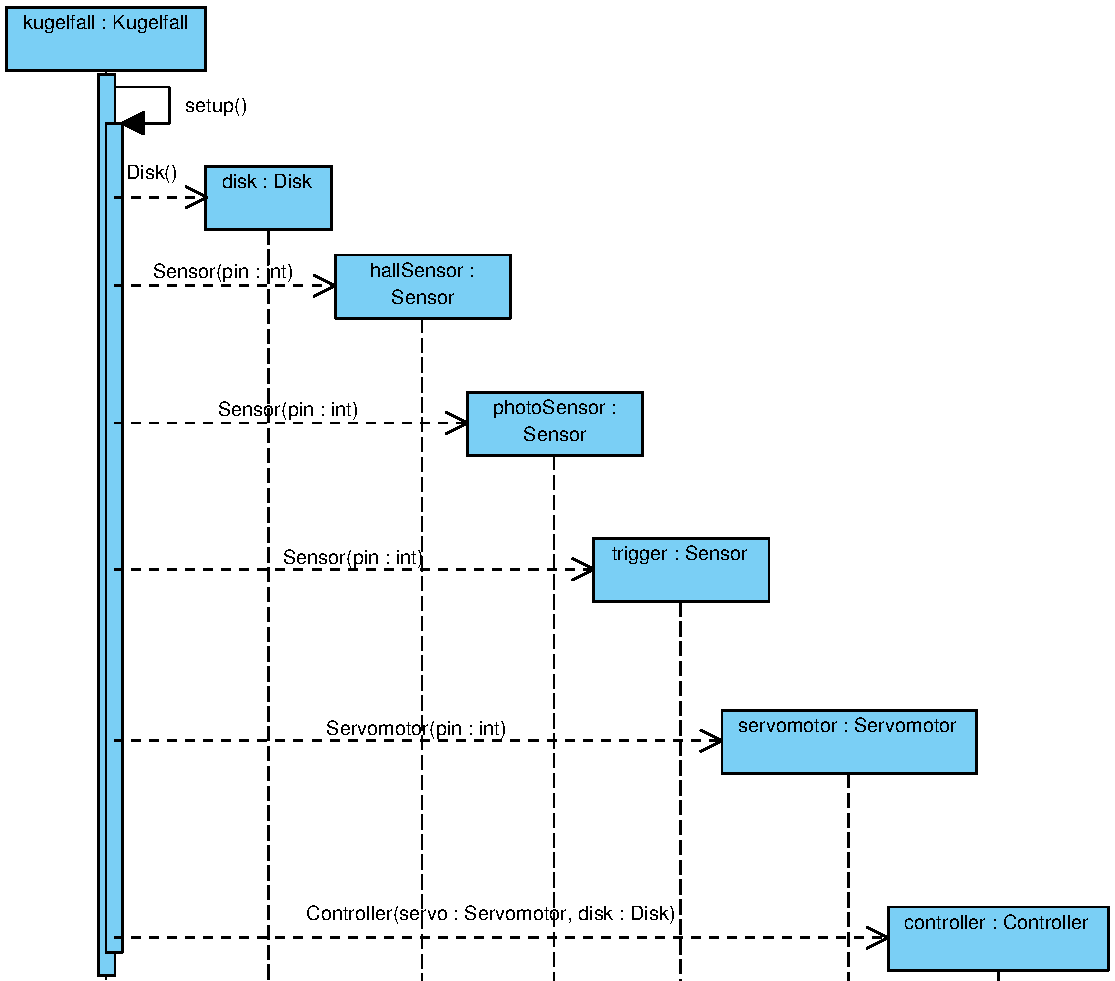
\includegraphics[width=\linewidth]{abb/setup_cropped}
	\caption{Ablauf bei der Methode \method{setup} von Klasse \class{Kugelfall}}
	\label{fig:setup_diagram}
\end{figure}
Dabei werden nacheinander die einzelnen Klassen instantiiert. 
Bei den Sensoren müssen die spezifischen Pins angegeben werden.
Bei der Initialisierung des \class{Controller} werden die Instanzen der Klassen \class{Servomotor} und \class{Disk} mit übergeben.

Diagramm \ref{fig:loop_diagram} zeigt den Ablauf in der Dauerschleife in der Methode \method{loop()}.
\begin{figure}[htbp]
	\centering
	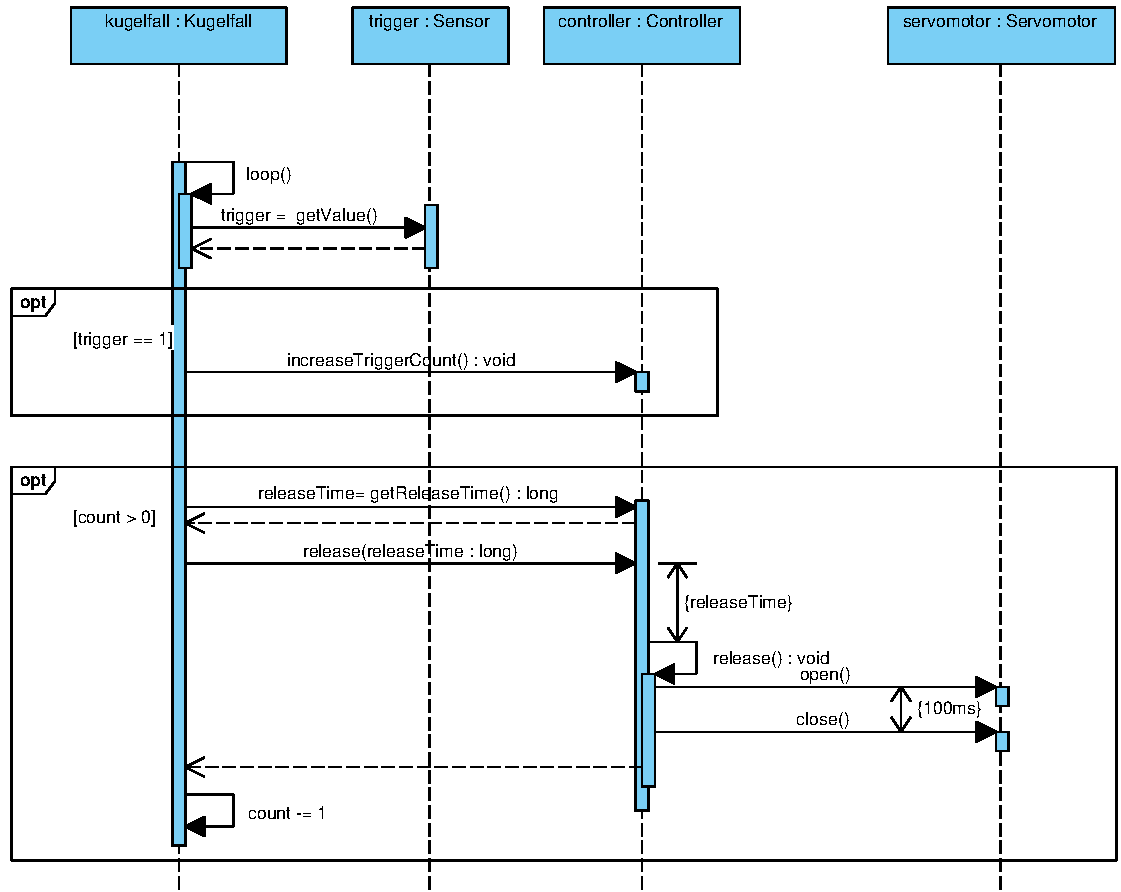
\includegraphics[width=\textwidth]{abb/loop_cropped}
	\caption{Ablauf bei der Methode \method{loop} von Klasse \class{Kugelfall}}
	\label{fig:loop_diagram}
\end{figure}
So wird zuerst der Triggerwert ausgelesen und damit geguckt, ob er vom Nutzer gedrückt wurde.
Ist das der Fall wird ein Triggerzähler im Controller um eins erhöht.
Ist der Zähler derzeit größer null wird die Berechnung der Fallzeit und das Loslassen der Kugel initialisiert.
So wird zuerst die Methode \method{getReleaseTime()} der Klasse \class{Controller} aufgerufen, welche die Zeit, bei welcher die Kugel fallengelassen werden soll, damit sie das Loch trifft, berechnet.
Danach wird die Methode \method{release()} mit der berechneten Zeit aufgerufen.
Diese wartet bis zur entsprechenden Zeit gewartet wird und lässt dann eine Kugel mittels der Methoden des \class{Servomotors} fallen.
Danach wird der Zähler wieder verringert.

Diagramm \ref{fig:photoISR} zeigt den Ablauf zum Festhalten der Messwerte des Photosensor mittels \method{photoISR()}. 
\begin{figure}[htbp]
	\centering
	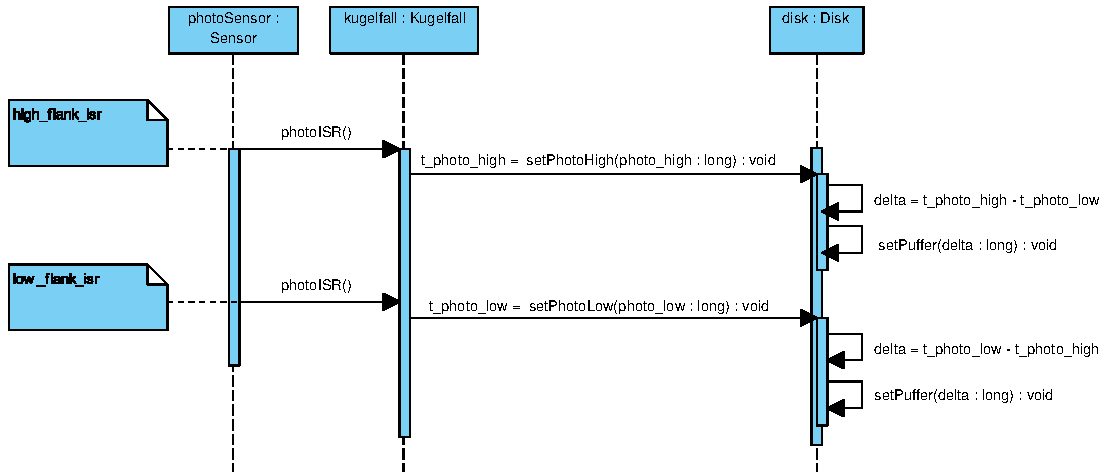
\includegraphics[width=\textwidth]{abb/photoISR_cropped}
	\caption{Ablauf bei der Methode \method{photoISR} von Klasse \class{Controller}}
	\label{fig:photoISR}
\end{figure}
So wird die  Methode \method{photoISR()} in Folge von steigenden und fallenden Flanken des Photosensor aufgerufen und die Werte mittels der Methode \method{setPhotoHigh()} bzw. \method{setPhotoLow} innerhalb eines Ringpuffers gespeichert.
Zur Unterscheidung der steigenden und fallenden Flanken dient die boolesche Variable \attr{isPhotoHigh}.
%Denn es stehen mit diesem Ringpuffer nicht nur auf der letzte Wert, sondern die letzten 20 Werte zur Verfügung.

Diagramm \ref{fig:hallISR} zeigt den Ablauf zum Festhalten der Messwerte des Hallsensor mittels \method{hallISR()}.
\begin{figure}[htbp]
	\centering
	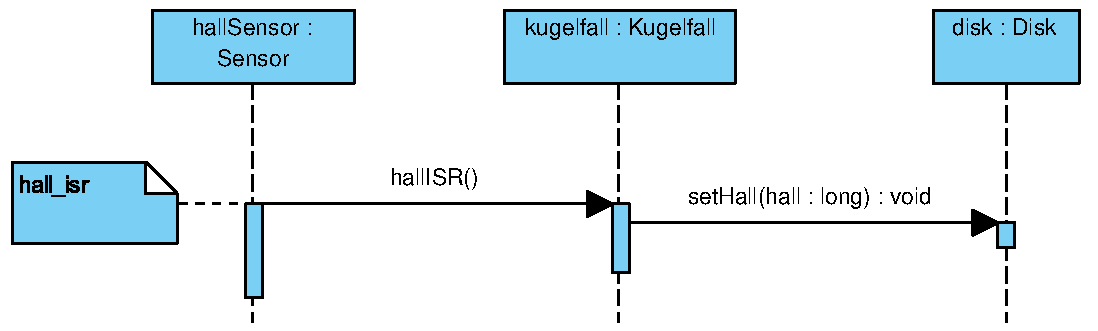
\includegraphics[width=0.8\textwidth]{abb/hallISR_cropped}
	\caption{Ablauf bei der Methode \method{hallISR} von Klasse \class{Controller}}
	\label{fig:hallISR}
\end{figure}
So wird die Methode \method{hallISR()} in Folge einer steigenden Flanke aufgerufen und die Werte Mittels der Method \method{setHall()} gespeichert.
Der Wert mittels \method{getHall()} ausgelesen werden.